\chapter{原子核}\label{chp:atomic_nucleus}
\section{天然放射现象}
\subsection{天然放射现象}
人类认识原子核的结构和它的变化规律,是从发现天然放射现象开始的。

1896 年,法国物理学家贝克勒耳(1852--1908)发现,铀和含铀的矿物能发出某种看不见的射线,这种射线可以穿透黑纸使照相底片感光。
物质发射这种射线的性质,叫做\Concept{放射性};具有放射性的元素,叫做\Concept{放射性元素}。

在贝克勒耳的建议下,玛丽·居里(1867--1934)和她的丈夫皮埃尔·居里(1859--1906)对铀和铀的各种矿石进行了深入的研究,并且发现了两种放射性更强的新元素。
玛丽·居里为了纪念她的祖国波兰,把其中一种元素命名为钋(读作“坡”,元素符号是 \ce{Po}),另一种命名为镭。

放射性并不是少数几种元素才有的,实际上原子序数大于 83 的所有天然存在的元素都具有放射性。
这种能自发地放出射线的现象叫做\Concept{天然放射现象}。

铀、钋和镭放出的射线到底是什么呢?
科学家们利用电场或磁场来研究放射线的性质,确定了放射线的组成。
\cref{fig:9-1} 表示利用电场进行研究的实验:把放射性样品放在铅块的窄孔底上,在孔的对面放着照相底片,没有电场时,在显影后的照相底片上可以发现正对着窄孔有一个暗斑,说明射线顺着窄孔一直射到底片上,使它感光。
在铅块和底片之间放上一对电极,使电场的方向跟射线的方向垂直时,在显影后的底片上出现三个暗斑,说明在电场作用下,射线分成三束(\cref{fig:9-1})。
其中有两束向相反方向偏转,表明这两束射线是由带电粒子组成的,而且两种粒子带有异种电荷;另外那束不发生偏转,表明这束射线是中性的。
从暗斑的位置知道,带正电的射线偏转较小,带负电的射线偏转较大。
通常把带正电的射线叫做 $\alpha$ 射线,带负电的射线叫做 $\beta$ 射线,不发生偏转的射线叫做 $\gamma$ 射线。

\begin{figure}
  \includegraphics{9-1.pdf}
  \caption{}\label{fig:9-1}
\end{figure}

卢瑟福对这些射线进一步研究,直接用实验证实 $\alpha$ 粒子带有两个单位的正电荷,质量数是 4\footnote{在原子核物理中,把基本电荷取作电荷的单位;把碳原子质量的 1/12 取作质量的单位,原子核的质量数通常非常接近整数,因此习惯上都用整数表示。}。$\alpha$ 粒子就是氦原子核。
$\alpha$ 粒子射出时的速度约为光速的十分之一。
$\alpha$ 射线贯穿物质的本领很小,在空气中只能飞行几厘米,一张薄铝箔或一张薄纸就能把它挡住;但是它有很强的电离作用,很容易使空气电离,使照相底片感光的作用也很强。
贝克勒耳用实验证实了 $\beta$ 射线是电子流,速度很接近光速。
$\beta$ 射线的贯穿本领很大,很容易穿透黑纸,甚至能穿透几毫米厚的铝板,但它的电离作用比较弱。
$\gamma$ 射线是一种波长很短的电磁波,它的贯穿本领最强,甚至能穿透几厘米厚的铅板,但它的电离作用却很小。

这三种射线都是从原子核里放射出来的,实验指出,当放射性物质连续发生衰变时,各种原子核中有的放射 $\alpha$ 射线,有的放射 $\beta$ 射线,同时伴随 $\gamma$ 射线,这时在放射线中就会同时有 $\alpha$、$\beta$、$\gamma$ 三种射线。
放射线的发现揭示了原子核结构的复杂性,从而促进了人类对微观结构的认识。

\subsection{放射性元素的衰变}

某元素的原子核,例如铀核,放出一个 $\alpha$ 粒子后,就变成了新的原子核。
我们把原子核由于放出某种粒子而转变为新核的变化叫做原子核的\Concept{衰变}。
在衰变中电荷数和质量数都是守恒的,我们用 \ce{^238_92U} 代表铀原子核,上标“238”表示核的质量数,下标“92”表示核的电荷数(可以省去下标,简写为 \ce{^238U},还可以简写为铀 238 或 U\,238)。
同样地,用 \ce{^4_2He} 代表氦原子核(即 $\alpha$ 粒子),用 \ce{^234_90Th} 代表钍原子核。
于是,\ce{^238_92U} 核放出 $\alpha$ 粒子变成 \ce{^234_90Th} 核的衰变可用下面的方程来表示:
\[ \ce{^238_92U -> ^234_90Th + ^4_2He}. \]
从这个方程可以看出,方程两边的质量数和电荷数都是相同的。
这种放出 $\alpha$ 粒子的衰变叫做 $\alpha$ 衰变。
$\alpha$ 衰变的规律是:新核的质量数比原来核的质量数减少 4,新核的电荷数比原来核的电荷数减少 2,因此新核在元素周期表中的位置要向前移两位,如果用 $M$ 表示核的质量数,$Z$ 表示核的电荷数,则 $\alpha$ 衰变的规律可以用下式表示(式中 \ce{X}、\ce{Y} 表示不同元素):
\[ ^{M}_{Z}\ce{X} \longrightarrow ^{M-4}_{Z-2}\ce{Y}+ \ce{^4_2He}.\]

\ce{^238_92U} 发生 $\alpha$ 衰变产生的 \ce{^234_90Th} 也具有放射性,它能放出一个 $\beta$ 粒子而变成 \ce{^234_91Pa}(镤)。
由于 $\beta$ 粒子就是电子,电子的质量比核的质量小得多,一个原子核放出一个 $\beta$ 粒子后,它的质量数不变,因此,可以认为电子的质量数是零,电荷数是 $-1$,于是我们用 \ce{^0_-1e} 来表示电子(即 $\beta$ 粒子)。
上述的衰变可表示为:
\[ \ce{ ^234_90Th -> ^234_91Pa + ^0_-1e}.\]
这个方程两边的质量数和电荷数也是相同的。
这种放出 $\beta$ 粒子的衰变叫做 $\beta$ 衰变,$\beta$ 衰变的规律是:新核的质量数不变,电荷数增加 1,新核在元素周期表中的位置要向后移一位,$\beta$ 衰变的规律可以用下式表示:
\[  ^{M}_{Z}\ce{X} \longrightarrow ^{M}_{Z+1}\ce{Y}+ \ce{^0_-1e}.\]

\subsection{半衰期}
放射性元素的衰变有一定的速率。例如,\ce{^222Rn} 经过 $\alpha$ 衰变变为 \ce{^218Po},如果隔一定时间测定一次剩余的氡的数量,就会发现,大约每过 \qty{3.8}{\text{天}},就有一半的氡发生了衰变。
也就是说,经过第一个 \qty{3.8}{\text{天}}以后,剩有一半的氡,经过第二个 \qty{3.8}{\text{天}}以后,剩有四分之一的氡,再经过 \qty{3.8}{\text{天}}以后,就只剩有八分之一的氡了。
因此,我们可以用\Concept{半衰期}来表示放射性元素衰变的速率:\emph{半衰期是放射性元素的原子核有半数发生衰变需要的时间}。
每一种放射性元素都有一定的半衰期,不同的放射性元素,半衰期不同,甚至差别非常大。例如前面说的 \ce{^222Rn}  变为 \ce{^218Po} 的半衰期是 \qty{3.8}{\text{天}},而 \ce{^226Ra} 变为 \ce{^222Rn} 的半衰期是 \qty{1620}{\text{年}},\ce{^238U} 变为 \ce{^234Th} 的半衰期竟长达 \qty{4.5e9}{\text{年}}!

放射性元素衰变的速率是由核内部本身的因素决定的,而跟原子所处的物理状态或化学状态无关。
例如,一种放射性元素,不管它是成单质存在或是成化合物存在,或者对它施加压力,或者增高它的温度,都不能改变它的半衰期。

\begin{Practice}
\begin{question}
  \item \ce{^230Th} 是 $\alpha$ 放射性的,它放出一个 $\alpha$ 粒子后变成了什么?写出衰变方程。
  \item \ce{^223Fr} 是 $\beta$ 放射性的,它放出一个 $\beta$ 粒子后变成了什么?写出衰变方程。
  \item \ce{^232Th} 经过六次 $\alpha$ 衰变和四次 $\beta$ 衰变后变成一种稳定的元素。这种元素是什么?它的原子量是多少?它的原子序数是多少?
  \item \ce{^238_92U} 变成 \ce{^206_82Pb},要经过几次 $\alpha$ 衰变和几次 $\beta$ 衰变?
  \item \ce{^210_83Bi} 的半衰期是 \qty{5}{d}。\qty{10}{g} 的 \ce{^210Bi} 经过 \qty{20}{d} 后还剩下多少?
  \item 放射性元素 \ce{^24_11Na} 经过 \qty{6}{h} 后只剩下 1/8 没有衰变,它的半衰期是多少?
\end{question}
\end{Practice}

\section{探测放射线的方法}
放射性元素放射出的 $\alpha$ 射线、$\beta$ 射线和 $\gamma$ 射线都是看不见的,需要根据它们跟其他物质作用产生的各种效应,用适当的仪器来探测。下面简单介绍三种方法。

\subsection{云室}
我们知道,水蒸气遇冷凝结,会形成很小的雾珠,这时它需要有凝结的核心,悬浮在空气中的尘埃微粒或气体离子都可以成为这种凝结核心。
云和雾就是这样形成的。
如果空气中没有任何尘埃或离子,水蒸气就是达到过饱和状态,也不能马上凝结。
但是,如果这时由于某种原因在空气中产生了离子,那么过饱和的水蒸气就会以这些离子为核心立即凝结成雾珠。
离子是看不见的,可是雾珠是看得见的,因此可以根据出现的雾珠来推测产生离子的情形。云室就是根据这个原理制成的。

\begin{figure}
  \includegraphics{9-2.pdf}
  \caption{云室}\label{fig:9-2}
\end{figure}

云室(\cref{fig:9-2})的主要部分是一个塑料或玻璃制的容器,它的下底是在小范围内可以上下移动的活塞,上盖是透明的,可以通过它来观察室内发生的现象或进行照相。
一小块放射性物质(放射源)放在室内侧壁附近(或放在室外,让放射线从侧壁的窗射入)。
实验时,先往云室里加一些酒精或乙醚(可以洒在云室下底上的黑绒布上),使室内充满酒精的饱和蒸气。
然后,使活塞突然迅速向下移动,室内气体由于迅速膨胀而降低温度,于是酒精蒸气达到过饱和。
这时如果有射线粒子从室内气体中飞过,使沿途的气体分子电离,过饱和的酒精蒸气就会以这些离子为核心凝结成一条雾迹。
这种云室是英国物理学家威耳逊(1869--1959)于 1911 年发明的,通常叫做威耳逊云室。

\begin{figure}
  \begin{minipage}{0.4\linewidth}\centering
    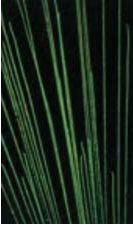
\includegraphics{9-3a.pdf}
    \subcaption{$\alpha$ 粒子}\label{fig:9-3a}
  \end{minipage}
  \begin{minipage}{0.4\linewidth}\centering
    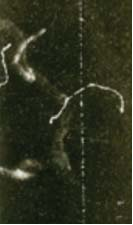
\includegraphics{9-3b.pdf}
    \subcaption{$\beta$ 粒子}\label{fig:9-3b}
  \end{minipage}
  \caption{云室中的径迹}\label{fig:9-3}
\end{figure}

用云室可以清楚地看出 $\alpha$ 粒子和 $\beta$ 粒子的径迹(\cref{fig:9-3})。$\alpha$ 粒子质量较大,在气体中行进时不易改变方向,它的电离本领大,在每厘米的路程中能使气体分子产生 \num{e4} 对离子,所以它的径迹直而粗。
$\beta$ 粒子质量很小,跟气体分子的电子碰撞时容易改变方向,而且电离本领小,在每厘米的路程中只能产生几百对离子,所以它的径迹比较细而且有时发生弯曲。
$\gamma$ 粒子电离本领更小,有时能产生一些细碎的雾迹。

\subsection{计数器}
计数器的主要部分是计数管,它是一支玻璃管,里面有一个导电的圆筒(或在管壁上涂一层导电薄膜)作阴极,一根通过圆筒轴心的金属丝作阳极(\cref{fig:9-4}),
\begin{figure}
  \includegraphics{9-4.pdf}
  \caption{计数管}\label{fig:9-4}
\end{figure}
管里装入惰性气体(如氩、氖等)和少量的乙醇汽或溴汽,气压大约是 \qtyrange{1.33e4}{2.66e4}{Pa}。
在两极加上大约 \qtyrange{800}{1500}{V} 的直流电压,这个电压略低于管内气体的击穿电压。
当有射线粒子飞进管内,使管内气体电离时,产生的电子在电场作用下向阳极加速运动。
电子在运动中能量越来越大,达到一定值时,跟气体分子碰撞,又可使气体分子电离,再产生电子,于是经过一段很短时间,就会产生大量电子,这些电子到达阳极,正离子到达阴极(正离子由于质量大,运动较慢,在运动中不会再使气体分子电离),就使计数管发生一次短暂的放电,从而得到一个脉冲电流。
这个脉冲电流可以用电子设备录下来。

这种计数器适合于对 $\beta$ 粒子和 $\gamma$ 粒子进行计数。
$\alpha$ 粒子的贯穿本领很小,要对它计数,需要在计数管上装一个很薄的窗口,或者制成其他式样。

\subsection{乳胶照相}
放射线能够使照相底片感光,放射线中的粒子经过照相底片上的乳胶时,使乳胶中的溴化银分解,经显影后,就有一连串的黑点显示出粒子的径迹。
这些径迹可用显微镜来进行观察与测量,根据径迹的长短和形状,可以判断入射粒子的性质、种类和能量。
乳胶的密度较大,粒子在乳胶中的射程约为空气中的千分之一,因此容易看到径迹的全部。
乳胶照相的主要优点是能够连续地工作,能够将入射粒子每个时刻的径迹记录下来。

随着科学技术的发展,探测射线的手段不断改进,近年来,由于探测仪器大都和电子计算机直接联结,实现了对实验全过程电子计算机控制、计算、数据处理,已经使实验方法高度自动化。

\section{原子核的人工转变\texorpdfstring{\quad}{ }原子核的组成}
放射现象的发现,使人们认识到原子核仍然具有内部结构,并且是能够发生变化的。
但是,能不能用人工的方法使原子核发生变化呢?原子核是由什么组成的呢?

\subsection{质子的发现}

1919 年,卢瑟福做了用 $\alpha$ 粒子轰击氮原子核的实验。
实验装置如\cref{fig:9-5} 所示。容器 $C$ 里放有放射性物质 $A$,从 $A$ 射出的 $\alpha$ 粒子射到一个铝箔 $F$ 上,适当选取铝箔的厚度;使 $\alpha$ 粒子恰好被它完全吸收,而不能透过,在 $F$ 的后面放一荧光屏 $S$,用显微镜 $M$ 来观察荧光屏上是否出现闪光。
通过阀门 $T$ 往容器 $C$ 里通入氮气后,卢瑟福从荧光屏 $S$ 上观察到了闪光,把氮气换成氧气或二氧化碳,又观察不到闪光。
这个实验表明,闪光一定是 $\alpha$ 粒子击中氮核后产生的新粒子透过铝箔引起的。
\begin{figure}
  \includegraphics{9-5.pdf}
  \caption{}\label{fig:9-5}
\end{figure}

后来,把这种粒子引进电场和磁场中,根据它在电场和磁场中的偏转,测出了它的质量和电量,确定它就是氢原子核,又叫做\Concept{质子},通常用符号 \ce{^1_1H} 或 \ce{^1_1p} 表示。
\begin{figure}
  \begin{minipage}[b]{0.4\linewidth}\centering
    \includegraphics{9-6a.pdf}
    \subcaption{}\label{fig:9-6a}
  \end{minipage}
  \begin{minipage}[b]{0.4\linewidth}\centering
    \includegraphics{9-6b.pdf}
    \subcaption{}\label{fig:9-6b}
  \end{minipage}
  \caption{}\label{fig:9-6}
\end{figure}

这个质子是 $\alpha$ 粒子直接从氮核中打出的,还是 $\alpha$ 粒子打进氮核后形成的复核发生衰变时放出的呢?
为了弄清这个问题,英国物理学家布拉凯特又在充氮的云室里做了这个实验。
如果质子是 $\alpha$ 粒子直接从氮核中打出的,那么在云室里就会看到四条径迹:入射 $\alpha$ 粒子的径迹,碰撞后 $\alpha$ 粒子的径迹,质子 $p$ 的径迹,抛出质子后的核的反冲径迹(\cref{fig:9-6a})。
如果 $\alpha$ 粒子打进氮核后形成一个复核,这复核立即发生衰变放出一个质子,那么在云室里就只能看到三条径迹;入射 $\alpha$ 粒子的径迹,质子 $p$ 的径迹,核的反冲径迹(\cref{fig:9-6b})。
布拉凯特拍摄了两万多张云室照片,终于从四十多万条 $\alpha$ 粒子径迹的照片中,发现有八条产生了分叉(\cref{fig:9-7})。
分叉的情况表明,上述的第二种设想是正确的。
从质量数守恒和电荷数守恒可以知道,这个新核是质量数等于 17 的氧。这个变化过程可以用下面的核反应方程来表示:
\[ \ce{ ^14_7 N + ^4_2 He -> ^17_8O + ^1_1 H }.\]
\begin{figure}
\includegraphics{9-7.pdf}
\caption{}\label{fig:9-7}
\end{figure}

在云室的照片中,分叉后细而长的是质子的径迹;短而粗的是反冲氧核的径迹。

后来,人们用同样的方法使氟、钠、铝等核发生了类似的转变,并且都产生了质子,由于从各种原子核里都能打出质子来,可见质子是原子核的组成部分。

\subsection{中子的发现}
卢瑟福用 $\alpha$ 粒子轰击氮核发现质子后,有人提出原子核可能是由带正电的质子组成的。
但这种设想遇到的困难是:除了氢原子外,所有元素的原子核的电荷数并不等于原子核的质量数。
例如,氦核的质量数是 4,电荷数是 2;\ce{^238U} 的质量数是 238,电荷数是 92。
那么原子核里除了质子外还有什么呢?

1920 年,卢瑟福曾预言:可能有一种质量与质子相近的不带电的中性粒子存在,他把它叫做\Concept{中子}。

1930 年发现,用由钋放出的 $\alpha$ 射线轰击铍(\ce{Be})时产生一种射线,这种射线的贯穿能力极强,它能够穿透几厘米厚的铅。当时,由被轰击物质产生的各种射线中,唯一能够贯穿铅层的是 $\gamma$ 射线,所以当时认为这种射线可能是 $\gamma$ 射线。

1932 年,约里奥·居里(1900--1958)和伊丽芙·居里(1897--1956)夫妇发现,如果用来自铍的这种射线去轰击石蜡(含有大量氢原子),竟能从石蜡中打出质子(\cref{fig:9-8})。
但从来也没有发现过 $\gamma$ 射线具有这样的性质,约里奥·居里夫妇想不出这种射线是什么。
\begin{figure}
  \includegraphics{9-8.pdf}
  \caption{}\label{fig:9-8}
\end{figure}

1932 年英国物理学家查德威克(1891--1974)仔细地研究了这种射线。
发现这种射线在磁场中不发生偏转,可见它是中性粒子流。
测出这种射线的速度不到光速的十分之一,因此排除了它是 $\gamma$ 射线的可能。
查德威克用这种射线轰击氢原子和氮原子。
结果打出了一些氢核(质子)和氮核。
他测量了被打出的氢核和氮核的速度,并由此推算出这种射线粒子的质量。

被打出的氢核的速度是不同的。
查德威克认为速度最大的氢核是由于未知射线中的粒子与它正碰的结果,其他速度较小的是由于斜碰的结果。
设 $m$ 是未知粒子的质量,$v$ 是它的速度,$m_\text{H}$ 是氢核的质量,$v'_\text{H}$ 是被打出的氢核的最大速度。
假定它们间的碰撞是弹性碰撞,氢核在未被打出前可以认为是静止的,根据高中一年级学过的弹性碰撞知识,我们知道,
\[ v'_\text{H}=\frac{2m}{m+m_\text{H}}v.\]

对于打出氮核的实验,设 $m_\text{N}$ 是氮核的质量,是被打出的氮核的最大速度,我们同样可以得到,
\[ v'_\text{N}=\frac{2m}{m+m_\text{N}}v.\]

我们知道,氮核的质量 $m_\text{N}$ 是氢核质量 $m_\text{H}$ 的 14 倍。把上述两式相除以消去未知的 $v$,并用 $14m_\text{H}$ 来代替 $m_\text{N}$,可得
\[ \frac{v'_\text{H}}{v'_\text{N}} =\frac{m+14m_\text{H}}{m+m_\text{H}}.\]

查德威克在实验中测得的氢核的最大速度是 \qty{3.3e9}{cm/s},氮核的最大速度是\qty{4.7e8}{cm/s}。把测得的数值代入上式进行计算,他得出 $m=1.15m_\text{H}$。

查德威克还用别的物质来代替氢和氮重做这个实验,得到的结果都是这种未知粒子的质量差不多等于氢核的质量。
这样,查德威克就发现了一种新的与氢核(质子)的质量差不多的粒子。
由于这种粒子不带电,所以叫做中子。

后来的更精确的实验测出,中子的质量非常接近于质子的质量,只比后者大千分之一多(中子的质量是 \qty{1.674920e-24}{g},质子的质量是 \qty{1.672614e-24}{g})。

在原子物理学中用 \ce{^1_0n} 表示中子,即中子的质量数是 1,电荷数是 0。
发现中子的核反应方程是
\[ \ce{ ^9_4Be +^4_2He -> ^12_6C +^1_0n}.\]

实验证实,从许多原子核里都能打出中子来,可见中子也是原子核的组成部分。

中子的发现是物理学史上的一件大事。
中子不带电荷,它与各种物质粒子不发生静电作用,很容易接近甚至打进原子核。
中子发现后,不少科学家用中子轰击原子核,进一步揭示了物质的微观结构,对近代物理的发展起了很大的作用。

\subsection{原子核的组成}

中子发现以后,如果认为原子核是由质子和中子组成的,以前在原子核结构理论中遇到的问题就可以解决了。
于是原子核是由质子和中子组成的看法,很快就得到了公认。

质子和中子统称为\Concept{核子}。
由于质子带一个单位的正电荷,中子不带电,质子和中子的质量几乎相等,都等于一个质量单位,所以原子核的电荷数就等于它的质子数,原子核的质量数就等于它的质子数与中子数的和。
具有相同质子数的原子,它们核外的电子数也相同,因而有相同的化学性质,属于同一种元素。
但它们的中子数可以是不同的,这些具有相同的质子数和不同的中子数的原子互称\Concept{同位素}。

在放射性元素的原子核中,2 个质子和 2 个中子结合在一起从核里发射出来,这就是 $\alpha$ 衰变。
原子核里虽然没有电子,但中子可以转化成质子和电子,这时产生的电子从核里发射出来,这就是 $\beta$ 衰变。
这一点,在后面\cref{sec:elemetary_particle}中还要说明。
至于 $\gamma$ 射线,是因为原子核中具有多余的能量而处于激发状态时,放出的射线。

\section{放射性同位素及其应用}
1934 年,约里奥·居里和伊丽芙·居里夫妇在用 $\alpha$ 粒子轰击铝箔时,除探测到预料中的中子外,还探测到了正电子。
正电子是物理学家在 1932 年发现的,它的质量跟电子的相同,带一个单位的正电荷,跟电子正好相反。
更意外的是,拿走 $\alpha$ 放射源以后,铝箔虽不再发射中子,但仍继续发射正电子,而且这种放射性随时间衰减的规律跟天然放射性一样,也有一定的半衰期。
原来,铝核被 $\alpha$ 粒子击中后发生了下面的反应:
\[ \ce {^27_13Al + ^4_2He -> ^30_15P +^1_0n }.\]
反应生成物 \ce{^30_15P} 是磷的一种同位素,它有放射性,象天然放射性元素一样发生衰变,衰变时放出正电子。
我们用符号 \ce{^0_1e} 表示正电子,于是 \ce{^30_15P} 的衰变反应可写为:
\[ \ce{ ^30_15P  -> ^30_14Si + ^0_1e}.\]

这种具有放射性的同位素,叫做\Concept{放射性同位素}。
用人工方法得到放射性同位素,这是一个很重要的发现。
后来用质子、氘核、中子和 $\gamma$ 光子轰击原子核,也得到了放射性同位素。
这样就进一步认识了原子核的性质,并知道了制造放射性同位素的方法。
天然放射性同位素只不过四十几种,而今天人工制造的放射性同位素已达一千多种,每种元素都有了放射性同位素。
于是放射性同位素在工业、农业、医疗卫生和科学研究的许多方面得到了广泛的应用。

放射性同位素的应用主要分为两类。
\subsubsection{利用它的射线}
例如利用 \ce{^60Co} 放出的很强的 $\gamma$ 射线来检查金属内部有没有砂眼或裂纹,这叫做 $\gamma$ 射线探伤(\cref{fig:9-9})。
用 $\gamma$ 射线比用 X 射线好,用 X 射线只能检查 \qtyrange{2}{3}{cm} 厚的钢板,并且 X 射线装置很复杂,使用也不方便。
用 $\gamma$ 射线可以检查 \qty{30}{cm} 厚的钢铁部件,放射性同位素还可以放进器件的内部,操作很方便。
\begin{figure}
  \includegraphics{9-9.pdf}
\caption{$\gamma$ 射线探伤的示意图}\label{fig:9-9}
\end{figure}

利用放射线的贯穿本领跟物体的厚度和密度的关系,可以用放射性同位素来检查各种产品的厚度、密封容器中的液面高度,从而自动控制生产过程。
\cref{fig:9-10} 是轧钢机上钢板厚度自动控制装置原理图。
让放射线穿过钢板射到探测器上,钢板的厚度发生变化时,透过钢板的射线的强度也随着变化,探测器把它转变为电信号输入到厚度指示装置和厚度控制装置,于是厚度指示装置就显示出厚度的变化,同时厚度控制装置自动地调整轧钢机上两轧辊的距离,使钢板的厚度恢复正常,从而保证钢板的厚度不超出公差的范围。
\begin{figure}
  \includegraphics{9-10.pdf}
  \caption{}\label{fig:9-10}
\end{figure}

在化纤、纺织等工业生产中,由于摩擦、分离等原因,织物和纤维上常聚集有害的静电。
将放射源放在容易产生静电的地方,放射性物质放出的射线可以使空气分子电离变成导电气体,这样可以把静电荷泄出。

用剂量不大的 $\gamma$ 射线照射植物(棉花、白菜、萝卜等)的种子能使产量显著增加。
利用射线可以防治害虫,射线照射能使幼虫失去发育能力,大剂量的照射能直接杀死害虫。
射线照射还能引起生物遗传特性发生突变以培育良种。
在医疗上射线可以使癌细胞受到抑制或死亡,因此常利用 \ce{^60Co} 的 $\gamma$ 射线来治疗肺癌、食道癌等。
射线还可以消毒灭菌,处理医院排除的污水,杀死各种病原体,保护环境卫生。
\subsubsection{做为示踪原子}
放射性同位素跟同种元素的非放射性位素的化学性质完全一样。
如果在某种元素里搀进一些放射性同位素,那么,无论这种元素走到哪里,它的放射性同位素也经历同样的过程。
由于放射性同位素会不停地放出放射线,用适当的探测仪器探测这些放射线,就会知道这种元素通过什么路径,运动到哪里了。
人们把作这种用途的放射性同位素叫做\Concept{示踪原子}。

示踪原子的应用是多方面的。
在内燃机工作时,活塞上的活塞环由于摩擦而磨损;如果使用带有放射性同位素 \ce{^59Fe} 的活塞环,这时具有放射性的 \ce{^59Fe} 被磨掉而混入润滑油中,测出油中的放射性就可以了解活塞环的磨损情况,而不必拆开内燃机去检查。
在农业施肥中,在肥料中加一些放射性同位素,就会知道哪种农作物在什么季节最能吸收含哪种元素的肥料。

在生物科学研究方面,同位素示踪技术也起着十分重要的作用。
我国科学家首先用人工方法合成了牛胰岛素,这是我国科学战线上的一项重大成就。
在这项工作中需要证明人工合成的牛胰岛素结晶跟天然牛胰岛素的结晶是同一种物质。
因此,在合成过程中搀入放射性\ce{^14C} 作示踪原子,然后把用 \ce{^14C} 标记的人工合成的牛胰岛素与天然牛胰岛素混合到一起,经过多次重新结晶后,得到了放射性 \ce{^14C} 分布均匀的牛胰岛素结晶,这就证明了人工合成的牛胰岛素与天然牛胰岛素完全融为一体,它们是同一种物质,从而为我国在国际上首先合成牛胰岛素提供了有力的证据。

放射线对人体组织是有伤害作用的,在使用放射性同位素时必须注意安全。要防止放射性物质对水源、空气、用具、工作场所的污染,并且要防止射线过多地照射人体。

\begin{Practice}
\begin{question}
  \item 用 $\alpha$ 粒子轰击氮核使它发生转变。从云室的照片中为什么可以确定细而长的径迹是质子产生的,粗而短的径迹是反冲氧核产生的。
  \item 用 $\alpha$ 粒子轰击氩 40,复核衰变时产生一个中子和一个反冲核,这反冲核是什么?写出核反应方程。
  \item 用 $\alpha$ 粒子轰击硼 10,产生一个中子和一个具有放射性的核,它是什么?这个核能放出正电子,它衰变后变成什么?写出核反应方程。
  \item 用中子轰击 \ce{^14N},产生 \ce{^14C},\ce{^14C} 具有 $\beta$ 放射性,它放出一个 $\beta$ 粒子后衰变成什么?写出核反应方程。
  \item 用中子轰击 \ce{^27Al},产生 \ce{^24Na},写出核反应方程。 \ce{^24Na} 是具有放射性的,衰变后变成 \ce{^24Mg},写出核反应方程。
  \item 带电的验电器在放射线照射下电荷会很快消失,说明原因。
\end{question}
\end{Practice}

\section{原子核的结合能}
\subsection{核力} 
原子核的半径很小,其中的质子之间的库仑斥力是很大的,然而通常的原子核却是很稳定的。
这表明,在原子核里,除了质子间的库仑力,还有另一种力,它把各种核子紧紧地拉在一起。
这种力叫做\Concept{核力}。
从实验知道,核力是一种很强的力,它在质子和质子间、质子和中子间、中子和中子间都存在,并且只在 \qty{2.0e-15}{m} 的短距离内起作用。
超过了这个距离,核力就迅速减小到零。
质子和中子的半径大约是 \qty{0.8e-15}{m},因此每个核子(质子或中子)只跟它相邻的核子间才有核力的作用。
核力只在很短的距离内发生作用,因此它既不是电磁力,也不是万有引力。关于核力的本质问题现在仍在深入研究中。

\subsection{结合能}
由于核子间存在强大的核力,所以原子核是一个坚固的集合体。要把原子核拆散成核子,需要克服核力做巨大的功,或者说需要巨大的能量。
例如,用强大的 $\gamma$ 光子照射氘核(它是由1个质子和一个中子组成的),可以使它分解为质子和中子,这时的核反应方程是:
\[ \gamma + \ce{ ^2_1H -> ^1_1H + ^1_0n}.\]
从实验知道,当光子能量小于 \qty{2.22}{MeV} 时,这个反应并不发生;只有光子的能量等于或大于 \qty{2.22}{MeV} 时,这个反应才会发生。
相反的过程,例如一个中子和一个质子结合成氘核,要放出 \qty{2.22}{MeV} 的能量,这个能量以 $\gamma$ 光子的形式辐射出去。这时的核反应方程是:
\[\ce{ ^1_0n + ^1_1H -> ^2_1H + }\gamma.\]

这表明,核子结合成原子核时要放出一定的能量;原子核分解成核子时,要吸收同样多的能量。
这个能量叫做原子核的\Concept{结合能}。

\subsection{质能方程\texorpdfstring{\quad}{ }质量亏损}

怎样才能求出原子核的结合能呢?虽然核力的本质还在研究之中,但是物理学家却有办法
求出结合能。
这要归功于大科学家爱因斯坦。
他从相对论得出质量和能量间有下述关系:
\[E=mc^2.\]
这个方程叫做爱因斯坦质能联系方程,简称\Concept{质能方程},式中 $c$ 是真空中的光速,$m$ 是物体的质量,$E$ 是物体的能量。
这个方程表明,物体的质量跟它的能量有一定的联系:物体的能量跟它的质量成正比,如果物体的能量增加了 $\Delta E$,物体的质量也相应地增加 $\Delta m$,反过来也一样。$\Delta E$ 和 $\Delta m$ 之间的关系符合爱因斯坦的质能方程
\[\Delta E=\Delta m\cdot c^2.\]

核子结合成原子核时要放出结合能,原子核的能量要比组成核的核子的能量小,所以原子核的质量也要比组成核的核子的质量小。
我们把组成原子核的核子的质量与原子核的质量之差叫做核的\Concept{质量亏损}。如果知道核的质量亏损,根据质能方程就可以求出核的结合能。

例如,氦核是由 2 个质子和 2 个中子组成的。每个质子的质量 $m_p$ 是 \qty{1.007277}{u},每个中子的质量 $m_n$ 是 \qty{1.008665}{u}。
氦核的质量 $m_{\alpha}$ 是 \qty{4.001509}{u}。
这里 \unit{u} 表示原子质量单位,$ \qty{1}{u}=\qty{1.660566e-27}{kg}$。
氦核的质量亏损 $\Delta m$ 可以计算如下:
\[\begin{split}
    2m_p&=2\times \qty{1.007277}{u}=\qty{2.014554}{u}\\
    2m_n&=2\times \qty{1.008665}{u}=\qty{2.017330}{u}\\
    m_{\alpha}&= \qty{4.001509}{u}\\
    \Delta m&=2m_p+2m_n-m_{\alpha}=\qty{0.030375}{u}\\
\end{split}\]

在原子核物理学中,核的结合能是用兆电子伏(\unit{MeV})来表示的。按照 $E=mc^2$ 可以求出,$\qty{1}{u}=\qty{931.5}{MeV}$。因此氦核的结合能是
\[ 0.030375 \times \qty{931.5}{MeV}=\qty{28.3}{MeV}.\]

\subsection{平均结合能} 
如果用核子数去除核的结合能,就得到每个核子的平均结合能。
对于氦来说,就是 $\qty{28.3}{MeV}/4=\qty{7.1}{MeV}$。
用同样的方法,可以求出其他原子核中每个核子的平均结合能。
平均结合能是核子结合成原子核时每个核子平均放出的能量,也是把原子核分解成核子时每个核子平均吸收的能量。
平均结合能越大,原子核就越难拆开。
可见平均结合能的大小能够反映核的稳定程度。
\cref{fig:9-11} 表示核子的平均结合能随原子核的质量数的变化规律。
图中的横坐标表示核的质量数,纵坐标表示核子的平均结合能。
从图中可以看出,质量数较小的轻核和质量数较大的重核,平均结合能都比较小。
中等质量数的原子核,平均结合能大。
质量数为 \numrange{50}{60} 的原子核,平均结合能最大,约为 \qty{8.6}{MeV}。
\begin{figure}
  \includegraphics{9-11.pdf}
  \caption{平均结合能曲线}\label{fig:9-11}
\end{figure}

\begin{Practice}
\begin{question}
  \item 氘核的质量是 \qty{2.013553}{u},根据质量亏损,计算氘核的结合能。
  \item 碳原子的质量是 \qty{12.000000}{u},可以看做是由 6 个氢原子(质量是\qty{1.007825}{u})和 6 个中子组成的。求碳原子核的结合能。(在计算中可以用碳原子的质量代替碳原子核的质量,用氢原子的质量代替质子的质量,因为电子的质量可以在相减过程中消去。)
  \item  在 \ce{^4_2He},\ce{^82_36Kr},\ce{^238_92U} 等原子核中核子的平均结合能个最大?哪个最小?原子核的结合能哪个最大?哪个最小?(根据平均结合能曲线进行比较)
  \item 如果要把 \ce{^16_8 O} 分成 8 个质子和 8 个中子,要给它多少能量?要把它分成 \ce{^4_2He},要给它多少能量?已知  \ce{^16_8 O} 的核子平均结合能是 \qty{7.98}{MeV},\ce{^4_2He} 的核子平均结合能是 \qty{7.07}{MeV}。
  \item 在一次核反应中,铀核 \ce{^235_92U} 变成了氙核 \ce{^136_54Xe} 和锶核 \ce{^90_38Sr}(同时放出了若干中子)。铀核的核子平均结合能约为 \qty{7.6}{MeV},氙核的核子平均结合能约为 \qty{8.4}{MeV},锶核的核子平均结合能约为 \qty{8.7}{MeV}。
  \begin{tasks}
    \task 把 \ce{^235U} 分解为核子,要吸收多少能量?
    \task 再使相应的核子分别结合成 \ce{^136Xe} 和 \ce{^90Sr},要放出多少能量?
    \task 在这个核反应中是吸收还是放出能量?这个能量大约是多大?
  \end{tasks}
\end{question}
\end{Practice}


\section{重核的裂变}
重核的核子平均结合能比中等质量的核的核子平均结合能小。
因此,重核分裂成中等质量的核时,会有一部分结合能释放出来。
这是释放原子核能——原子能的一种重要方法。
这种核反应叫做\Concept{裂变}。

\subsection{铀核的裂变}
重核的裂变是在本世纪三十年代末期用中子轰击铀核时发现的。
铀核裂变的产物是多种多样的,有时裂变为氙(\ce{Xe})和锶(\ce{Sr}),有时裂变为钡(\ce{Ba})和氪(\ce{Kr})或锑(\ce{Sb})和铌(\ce{Nb}),同时放出 \numrange{2}{3} 个中子,铀核还可能分裂成三部分或四部分,不过这种情形比较少见。

铀核的裂变过程,可以用下面的示意图来说明(\cref{fig:9-12})。
\begin{figure}
\includegraphics{9-12.pdf}
\caption{}\label{fig:9-12}
\end{figure}

当中子打进 \ce{^235U} 后,就形成处于激发状态的复核,复核中的核子由于激烈运动,使核变成不规则形状,核子间的距离增大。
由于核力只在极短距离内发生作用,当核子间距离增大时,核力迅速减小,因而不能克服质子间的库仑斥力使核恢复原状,核就分裂成两部分,同时放出几个中子。

铀核裂变的许多可能的核反应中的一个是:
\[ \ce{^235_92U +^1_0n -> ^141_56Ba +^92_36Kr + 3 ^1_0n },\]
在这个反应中释放的能量可以计算如下:裂变以前:
\[\qty{235.0439}{u}+\qty{1.0087}{u}=\qty{236.0526}{u},\]
裂变以后:
\[\qty{140.9139}{u}+\qty{91.8973}{u}+\qty{3.0261}{u}=\qty{235.8373}{u},\]
反应过程中质量减少 $\Delta m=\qty{0.2153}{u}$,反应中释放的能量
\[\Delta E=\Delta m\cdot c^2=\qty{201}{MeV}.\]
在不同的反应中,铀核释放的能量也不同。
如果按照一个铀核裂变时放出 \qty{200}{MeV}的能量来估算,\qty{1}{kg} 铀全部裂变时放出的原子能就相当于 \qty{2500}{t} 优质煤完全燃烧时放出的化学能。

\subsection{链式反应} 
铀核裂变时,同时放出 \numrange{2}{3} 个中子,如果这些中子再引起其他铀核裂变,就可使裂变反应不断地进行下去。
这种反应叫做链式反应(\cref{fig:9-13})。
\begin{figure}
  \includegraphics{9-13.pdf}
  \caption{链式反应}\label{fig:9-13}
\end{figure}

在天然铀中,主要有两种同位素,其中 99.3\% 是 \ce{^238U},0.7\% 是 \ce{^235U}。
这两种铀跟中子的作用很不相同。
\ce{^235U} 俘获各种能量的中子都会发生裂变,而且俘获能量低的中子发生裂变的几率较大。
\ce{^238U} 只有俘获能量大于 \qty{1}{MeV} 的中子才可能发生裂变,并且几率很小。
它俘获能量低于 \qty{1}{MeV} 的中子时不发生裂变,而变成 \ce{^239U}。
能量低于 \qty{1}{eV} 的中子跟 \ce{^238U} 基本上只发生弹性碰撞,不引起核反应。
因此,为了使裂变的链式反应容易发生,最好是利用纯 \ce{^235U}。

铀块的体积对于产生链式反应也是一个重要因素。
因为原子核非常小,如果铀块的体积不够大,中子从铀块中通过时,可能还没有碰到铀核就跑到铀块外面去了。
能够发生链式反应的铀块的最小体积叫做它的\Concept{临界体积}。

如果 \ce{^235U} 的体积超过了它的临界体积,只要有中子进入铀块,会立即引起铀核的链式反应,在极短时间内就会释放出大量的核能,发生猛烈的爆炸。
原子弹就是根据这个原理制成的。

\subsection{核反应堆}
核反应堆是用人工控制链式反应的装置。
原子弹爆炸时链式反应的速度是无法控制的,为了用人工方法控制链式反应的速度,使核能比较平缓地释放出来,人们制成了核反应堆。
\begin{figure}
  \includegraphics[scale=1.2]{9-14.pdf}
  \caption{原子反应堆示意图}\label{fig:9-14}
\end{figure}

\cref{fig:9-14} 是原子反应堆的示意图。
反应堆里用的铀棒是天然铀或浓缩铀(其中 \ce{^235U} 的含量比天然铀高)。
由于裂变产生的是速度很大的快中子,很容易被 \ce{^238U} 俘获而不发生裂变,所以必须设法使中子在碰上 \ce{^238U} 前降低速度。
为此在铀棒的周围放上原子量比较小、又不吸收或很少吸收中子的物质,如石墨、重水或普通水(普通水吸收中子的几率较大,但可以用在以浓缩铀做原料的反应堆中),快中子跟这些物质的原子核碰撞后,能量减小,变成慢中子。
这种用来使中子减速的物质叫做\Concept{减速剂}。
速度跟热运动速度差不多的慢中子(能量约为 \qty{2.5e-2}{eV})叫做热中子。
热中子碰到 \ce{^238U} 时会弹射回来,却容易被 \ce{^235U} 俘获而引起裂变。
为了调节中子数目以控制反应速度,还需要在铀棒之间插进一些镉棒。
镉吸收中子的能力很强,当反应过于激烈时,使镉棒插入深一些,让它多吸收一些中子,链式反应的速度就会慢一些;当反应过于缓慢,达不到所需功率时,使镉棒插入浅一些,让它少吸收一些中子,链式反应速度就可以增大。
这种镉棒叫做\Concept{控制棒}。
用电子仪器自动地调节控制棒的升降,就能使反应堆保持一定的功率安全地工作。

反应堆工作时,核燃料裂变释放出的核能转变为热能,使反应堆的温度升高。
为了控制反应堆的温度,使它能正常工作,需要用水、液体金属钠或空气等流体作冷却剂,在反应堆内外循环流动,不断地带走热能。
这就是反应堆的冷却系统,它同时可以用来输出热能。

为了防止铀核裂变物放出的各种射线对人体的危害,在反应堆的外面需要修建很厚的水泥防护层,用来屏蔽射线,不让它们透射出来。
对放射性的废料,也要装入特制的容器,埋入深地层进行处理。

利用反应堆工作时释放出的热能使水汽化以推动汽轮发电机发电,这就是核电站。\cref{fig:9-15} 是核电站示意图。
核电站消耗的“燃料”很少。
一座一百万千瓦的核电站,每年只消耗 \qty{30}{t} 浓缩铀,而同样功率的火力发电站,每年却要消耗 \qty{250e4}{t} 煤。
目前,核能发电的经济效益跟火电站大体相同。
到 1983 年底、核发电已占世界发电总量的 12\%。
为了适应我国现代化建设对能源日益增长的需要,在广东、浙江、江苏、辽宁等省正在建造核电站。

\begin{figure}
  \includegraphics{9-15.pdf}
  \caption{核电站示意图}\label{fig:9-15}
\end{figure}

原子能反应堆不仅可以提供强大的原子能,而且它产生的大量中子还可以用来进行各种原子核物理实验,制造各种放射性同位素。

利用原子能反应堆还可以生产新的核燃料。
从实验知道,快中子被 \ce{^238U} 俘获后,变成 \ce{^239U}, \ce{^239U} 是不稳定的,经过两次 $\beta$ 衰变后变成 \ce{^239Pu}。
\ce{^232Th} 与中子作用后,经过两次 $\beta$ 衰变后变成 \ce{^233U}。
\ce{^239Pu} 和 \ce{^233U} 的性质跟 \ce{^235U} 一样,很容易俘获中子而发生裂变,因此也可以作为供裂变用的核燃料。
因此,如果在反应堆中装入 \ce{^238U} 或 \ce{^232Th},并设法使每一次核裂变能够产生一个以上的 \ce{^239Pu} 或 \ce{^233U},那么,我们就可以使新产生的核燃料多于消耗的核燃料,使 \ce{^238U} 和 \ce{^232Th} 也可以得到利用,这种反应堆叫做增殖反应堆。
地球上的 \ce{^238U} 和 \ce{^232Th} 的总量大约是 \ce{^235U} 的 800 倍,建造增殖反应堆可以利用 \ce{^238U} 和 \ce{^232Th},更有效地利用核资源。
增殖反应堆虽然处于试验阶段,但从长远来看是很有前途的。

\section{轻核的聚变}
\subsection{聚变}
轻核的结合能更小,某些轻核结合成质量较大的核时,能释放出更多的结合能。
例如:一个氘核和一个氚核结合成一个氨核时,释放出 \qty{17.6}{MeV} 的能量,平均每个核子放出的能量在 \qty{3}{MeV} 以上,这时的核反应方程是
\[ \ce{ ^2_1H + ^3_1H -> ^4_2He + ^1_0n }.\]
轻核结合成质量较大的核叫做\Concept{聚变}。

使核发生聚变,必须使它们接近到 \qty{e-15}{m},也就是接近到核力能够发生作用的范围。
由于原子核都是带正电的,要使它们接近到这种程度,必须克服电荷之间的很大的斥力作用。
这就要使核具有很大的动能。
用什么办法能使大量的轻核获得足够的动能来产生聚变呢?
有一种办法,就是把它们加热到很高的温度。
从理论分析知道,物质达到几百万度以上的高温时,原子的核外电子已经完全和原子脱离,这时小部分原子核就具有足够的动能,能够克服相互间的库仑斥力,在互相碰撞中接近到可以发生聚变的程度。
因此,这种反应又叫做\Concept{热核反应}。
怎样产生这样高的温度呢?我们知道,原子弹爆炸时能产生这样高的温度,所以可以用原子弹来引起热核反应。
氢弹就是这样制造出来的。

热核反应在宇宙中是很普遍的现象。
在太阳内部和许多恒星内部,温度都高达 1 千万度以上,在那里热核反应激烈地进行着。
太阳每秒钟辐射出来的能量约为 \qty{3.8e26}{J},就是从热核反应中产生的。
地球只接受了其中的二十亿分之一,就使地面温暖,产生风云雨露,河川流动,生物生长。

\subsection{可控热核反应}
原子弹、氢弹虽然能够引起热核反应释放出巨大能量,但能量是瞬时释放出来的。
和平利用核能则需要聚变能缓慢而稳定的释放,释放的速率应当能够被人控制,即发生可控热核反应,这种反应就是用人工的办法,有控制地使氘核产生聚变反应,从而释放出能量。
热核反应需要的原料——氘,在世界上的储量是非常丰富的。
\qty{1}{L} 海水中大约有 \qty{0.03}{g} 的氘,如果用来发生热核反应,它放出的能量就和燃烧 \qty{300}{L} 汽油相当。
因此海水中的氘就是异常丰富的能源。

热核反应除了原料丰富外,还有以下几个特点:它释放出的能量,就每一个核子平均来说,比裂变反应要大好几倍。
而且裂变反应会产生带有强放射性的物质,对环境造成放射性污染;热核反应对环境的污染要轻得多,也比较容易处理。
从热核反应中还可以得到大量有用的中子。
可控热核反应是核能利用的一条途径,受到普遍重视。

目前,世界上许多国家,都在积极研究可控热核反应的理论和技术。
我国自行设计和制造的可控核聚变实验装置“中国环流器一号”已于 1984 年 9 月顺利启动。
它标志着我国研究可控热核聚变的实验手段有了新的发展和提高,必将为人类探求新能源作出贡献。

\section{基本粒子}\label{sec:elemetary_particle}
直到十九世纪末,人们都认为原子是组成物质的最小的不可再分的微粒。后来发现了电子、质子和中子,并且知道了质子和中子组成了原子核,原子核和电子组成了原子,这时许多人又认为电子、质子和中子是组成物质的最基本的粒子,把它们叫做\Concept{基本粒子}。

随着科学技术的发展,从二十世纪三十年代以来,人们不断地从宇宙射线和原子核物理实验中发现了大量的基本粒子。

宇宙射线是从宇宙空间射来的高能粒子,其中主要是质子,还有少量的 $\alpha$ 粒子和其他粒子。
这些粒子的能量很高,大部分高达 \qtyrange{e9}{e10}{eV},少数粒子具有更高的能量。
宇宙射线进入地球大气层后,跟大气中的原子核碰撞,会引起很多种核反应,产生各种核反应产物。
自从 1911 年发现宇宙射线以后,就开始了对宇宙射线的观测。
在宇宙射线的研究中,陆续发现了一些新的基本粒子:1932 年发现正电子,1937 年发现 $\mu$ 介子(后来称为 $\mu$ 子),1947年又发现 K 介子和 $\pi$ 介子。
这些介子的质量是介于质子和电子之间的,因此叫做\Concept{介子}。
后来又发现了质量比质子大的粒子,名叫\Concept{超子}\footnote{六十年代以后,又发现了质量比质子大的介子,因此介子、超子这些名称只具有历史上的意义。}。

1932 年发明了回旋加速器,后来建成了各种加速器。
在用加速器进行的实验中,发现了更多的基本粒子。
并且发现,许多粒子都有和它的质量相同而电荷相反的粒子,叫做\Concept{反粒子}。
例如,电子的反粒子就是正电子,正 $\pi$ 介子的反粒子就是负 $\pi$ 介子。
质子的反粒子叫做反质子,是 1955 年发现的,它带有单位负电荷,现在发现的基本粒子已达几百种。

按照基本粒子之间的相互作用,可以把它们分为三类:

\begin{description}
  \item[强子] 核子之间的核力是一种比电磁作用大得多的相互作用,叫做\Concept{强相互作用}。凡是参与强相互作用的粒子,都叫做强子。目前发现的基本粒子,绝大多数是强子。质子是最早发现的强子,强子又分重子(中子、质子、超子)和介子两类。
  \item[轻子] 都不参与强相互作用,只发现几种。电子是最早发现的轻子。$\mu$ 子从它的许多性质来看属于轻子。1975 年,又发现了一种质量很大的轻子,称为 $\tau$ 子,也叫重轻子。
  \item[媒介子] 是传递粒子间相互作用的粒子,例如光子就是其中的一种,是传递电磁相互作用的。
\end{description}

\bigskip
绝大多数基本粒子都是不稳定的,在很短时间内就发生衰变,并且能相互转变。例如,正负 $\pi$ 介子的平均寿命约为 \qty{2.6e-8}{s},它衰变为 $\mu$ 子,同时产生一种质量非常小(与电子质量相比,可以认为质量为零)的中性粒子,叫做\Concept{中微子},它属于轻子,用 $\nu$ 表示。$\mu$ 子也是不稳定的,平均寿命约为 \qty{2.2e-6}{s},衰变为电子和正反两个中微子。

中子也可以转化,自由状态的中子的平均寿命约为 \qty{16}{min},它衰变为一个质子、一个电子和一个反中微子;
\[ \ce { ^1_0n -> ^1_1p + ^0_-1e + } \bar{\nu}.\]
放射性原子核的 $\beta$ 衰变,实际发生的就是这种反应,由中子转化成的质子仍留在原子核内,同时产生的电子(即 $\beta$ 粒子)和反中微子则放射出去。

质子在自由状态是稳定的,但在原子核内也会转化为一个中子,同时放出一个正电子和一个中微子:
\[\ce{ ^1_1p -> ^1_0n + ^0_1e }+ \nu.\]
放射性同位素 \ce{^30P} 的衰变,实际发生的就是这种反应。

一对正反粒子相遇时,会同时消失而转化为别种粒子,这种现象叫做\Concept{湮灭}。例如,一个电子和一个正电子相遇会发生湮灭而转化为一对光子:
\[ \ce{ ^0_-1e +^0_1e -> } \gamma + \gamma .\]

相反的过程也能够发生。
例如,能量超过 \qty{1.02}{MeV} 的 $\gamma$ 光子穿过铅板时,会同时产生电子和正电子,通常把这一对正负电子叫做电子—正电子偶。
\cref{fig:9-16} 是在云室中看到的它们的径迹,由于电子和正电子所带的电荷相反,它们在磁场中向相反的方向偏转,这个反应可表示为:
\[ \gamma \ce{ -> ^0_-1e +^0_1e }.\]
这些事实表明,光子和电子虽然有基本的区别,但是仍然有着深刻的联系。
\begin{figure}
  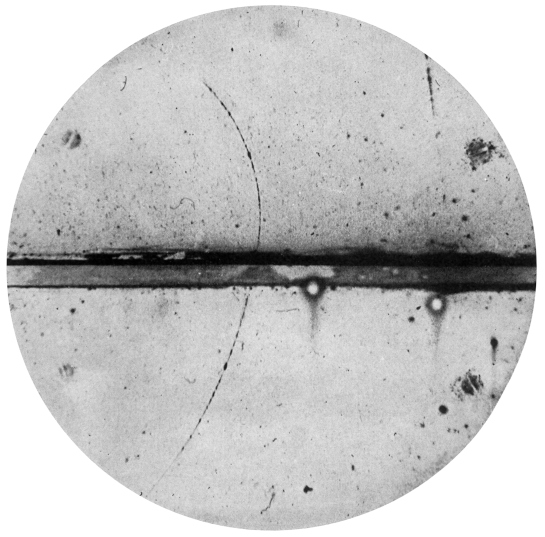
\includegraphics{9-16.jpg}
  \caption{电子—正电子偶的径迹}\label{fig:9-16}
\end{figure}

基本粒子的种类这样多,并且能够相互转化,这就促使人们进一步去研究基本粒子的结构。
许多实验事实表明,强子是有内部结构的。
因此许多物理学家倾向于不再使用“基本粒子”这个名称,而改称为“粒子”。
为了探索强子的内部结构,先后提出了多种模型,其中比较成功的是\Concept{夸克模型},认为强子是由夸克(我国也叫层子)组成的。
目前,这个模型里有六类(共十八种)夸克,还有同样数目的反夸克,它们所带的电荷是基本电荷的 $\pm \frac{1}{3}$ 或 $\pm\frac{2}{3}$。
重子是由三个夸克组成的,反重子是由三个反夸克组成的,介子是由一个夸克和一个反夸克组成的。
从夸克理论得出的许多结果都跟实验符合得很好。
但在实验中还没有发现自由夸克。
关于夸克模型的理论正在进一步发展中。

物质世界,无论从宏观方面看,还是从微观方面看,都是无穷尽的,人类对物质世界的认识将一步一步地深人,永远不会终止。
关于基本粒子的物理学——高能物理正在蓬勃发展中,人们终将认识基本粒子的结构和变化规律。

\begin{Review}
\begin{question}
  \item 什么是放射性元素?$\alpha$ 射线、$\beta$ 射线、$\gamma$ 射线的本质是什么?三种射线各有什么特性?
  \item 什么是 $\alpha$ 衰变?$\alpha$ 衰变的规律是什么?什么是 $\beta$ 衰变?$\beta$ 衰变的规律是什么?什么是半衰期?
  \item 说明用云室、计数器、乳胶照相探测射线的基本原理。
  \item 什么是质子?质子是怎样发现的?什么是中子?中子是怎样发现的?原子核是怎样组成的?什么是同位素?
  \item 简述放射性同位素有哪些应用。
  \item 什么是原子核的结合能?什么是爱因斯坦的质能方程?怎样根据质能方程计算结合能?什么是平均结合能?平均结合能的大小反映核的什么性质?
  \item 什么是重核的裂变?什么是链式反应?在核反应堆中怎样控制裂变的速度?
  \item 什么是轻核的聚变?产生聚变的条件是什么?研究可控热核反应有什么意义?
  \item 简述基本粒子的种类。
\end{question}
\end{Review}

\begin{Exercise}*
\begin{question}
  \item \ce{^238U} 的半衰期是 \qty{4.5e9}{\text{年}},假设一块矿石中含有 \qty{1}{kg} 的 \ce{^238U} ,经过 45 亿年(相当于地球的年龄)以后,还剩有多少铀 238?假设发生衰变的 \ce{^238U}  都变成了 \ce{^206Pb} ,矿石中会有多少铅?这时铀铅的比例是多少?再经过 45 亿年,矿石中的铀铅比例将变成多少? 根据这种铀铅比例能不能判断出矿石的年龄?
  \item 镭核在 $\alpha$ 衰变中放出能量为 \qty{4.78}{MeV} 的 $\alpha$ 粒子和能量为 \qty{0.19}{MeV} 的 $\gamma$ 粒子。如果 \qty{1}{g} 镭每秒钟有 \num{3.7e10} 个原子核发生 $\alpha$ 衰变,算出它每秒钟释放多少能量。
  \item 静止状态的放射性原子核镭(\ce{^226_88Ra})进行 $\alpha$ 衰变。为了测量 $\alpha$ 粒子的动能 $E$,让 $\alpha$ 粒子垂直飞进 $B=\qty{1}{T} $ 的匀强磁场,测得 $\alpha$ 粒子的轨道半径 $r=\qty{0.2}{m}$。
  \begin{tasks}
    \task 写出 \ce{Ra}的 $\alpha$ 衰变方程。
    \task 试计算 $\alpha$ 粒子的动能 $E$。
  \end{tasks}
  \item 在某些恒星内,三个 $\alpha$ 粒子结合成一个 \ce{^12_6C} 核。\ce{^12_6C} 的质量是 \qty{12.0000}{u},\ce{^4_2He} 的质量是 4.0026u。这个反应中放出多少能量?
  \item 已知 \ce{^226_88Ra},\ce{^222_86Rn},\ce{^4_2He} 的原子量分别是 226.0254,222.0175,4.0026。求在 \ce{^226_88Ra} 衰变
  \[ \ce{ ^226_88Ra -> ^222_86Rn + ^4_2He}\]
  中放出的能量是多少电子伏?如果这些能量都以 \ce{Rn} 核和 \ce{He}核 的动能形式释放出来,放出的 $\alpha$ 粒子的速度有多大?

  提示:能量和动量都守恒。
  \item 在一原子反应堆中,用石墨(碳)作减速剂使快中子减速。已知碳核的质量是中子的 12 倍,假设把中子与碳核的每次碰撞都看作是弹性正碰,而且认为碰撞前碳核都是静止的。
  \begin{tasks}
    \task 设碰撞前中子的动能是 $E_0$,经过一次碰撞,中子损失的能量是多少?
    \task 至少经过多少次碰撞,中子的动能才能小于 $10^{-6}E_0$?
  \end{tasks}
\end{question}
\end{Exercise}
